\documentclass[11pt, addpoints, answers]{exam}

\usepackage{amsmath, amssymb}
\usepackage{xcolor}
\usepackage{tikz}
\usepackage{enumerate}
\usepackage{graphicx}
\usepackage{tabularx}
\usepackage{algorithm}
\usepackage{algpseudocode}
\usepackage{tikz}

\newcommand{\red}[1]{\textcolor{red}{#1}}
\newcommand{\blue}[1]{\textcolor{blue}{#1}}

% For inserting code snippets.
\usepackage{listings}
\lstset{
    columns = fixed,
    basewidth = {0.5em},
    breaklines = true,
    backgroundcolor = \color{white},
    keywordstyle = \color[RGB]{40, 40, 255},
    numberstyle = \footnotesize\color{darkgray},
    commentstyle = \ttfamily\color{violet},
    basicstyle = \ttfamily,
    stringstyle = \ttfamily\color[RGB]{128, 0, 0},
    showstringspaces = false,
    language = {[11]C++},
    escapechar = \@
}
\lstnewenvironment{cpp}[1][]{\lstset{language = {[11]C++}, #1}}{}

\renewcommand{\baselinestretch}{1.15}
\setlength{\parskip}{1.25\baselineskip}

% headers, footers, titles
\newcommand{\CourseName}{CS101 Algorithms and Data Structures}
\newcommand{\HomeworkNO}{5}
\newcommand{\DueDate}{November 6, 2024}

\pagestyle{headandfoot}
\runningheadrule
\runningheader{CS101 Fall24}{Homework \HomeworkNO}{Due on: \DueDate}
\runningfooter{}{\thepage}{}

\title{
    \vspace{25pt}
    \LARGE ShanghaiTech University \\
    \bigskip
    \textbf{\CourseName} \\
    \textbf{Fall 2024}   \\
    \bigskip
    Homework \HomeworkNO
}
\author{}
\date{Due date: \DueDate, at 23:59}

% formats of questions, choices, points, etc.
\qformat{\bf\thequestion. (\totalpoints\ points) \thequestiontitle\hfill}
\pointname{'}
% \CorrectChoiceEmphasis{\bf\color{blue}}
% \SolutionEmphasis{\color{blue}}

% We frequently use this font.
\newcommand{\ttt}{\texttt}
\newcommand{\bluett}[1]{\textcolor{blue}{\ttt{#1}}}

\begin{document}

\maketitle

\vspace{50pt}

\begin{enumerate}
    \item Please write your solutions in English.
    \item Submit your solutions to Gradescope.
    \item Set your FULL name to your Chinese name and your STUDENT ID correctly in Gradescope account settings.
    \item If you want to submit a handwritten version, scan it clearly. \ttt{CamScanner} is recommended.
    \item We recommend you to write in \LaTeX.
    \item When submitting, match your solutions to the problems correctly.
    \item No late submission will be accepted.
    \item Violations to any of the above may result in zero points.
\end{enumerate}

\begin{questions}

\newpage
\titledquestion{Multiple Choices}

Each question has \textbf{one or more} correct answer(s). Select all the correct answer(s). For each question, you will get 0 points if you select one or more wrong answers, but you will get 1 point if you select a non-empty subset of the correct answers.

Write your answers in the following table.

%%%%%%%%%%%%%%%%%%%%%%%%%%%%%%%%%%%%%%%%%%%%%%%%%%%%%%%%%%%%%%%%%%%%%%%%%%%
% Note: The `LaTeX' way to answer a multiple-choices question is to replace `\choice'
% with `\choice', as what you did in the previous questions. However, there are 
% still many students who would like to handwrite their homework. To make TA's work 
% easier, you have to fill your selected choices in the table below, no matter whether 
% you use LaTeX or not.
%%%%%%%%%%%%%%%%%%%%%%%%%%%%%%%%%%%%%%%%%%%%%%%%%%%%%%%%%%%%%%%%%%%%%%%%%%%

\begin{table}[htbp]
	\centering
	\begin{tabular}{|p{1.7cm}|p{1.7cm}|p{1.7cm}|p{1.7cm}|p{1.7cm}|p{1.7cm}|p{1.7cm}|p{1.7cm}|p{1.7cm}|}
		\hline
		(a) & (b) & (c) & (d) & (e) & (f) \\
		\hline
		%%%%%%%%%%%%%%%%%%%%%%%%%%%%%%%%%%%%%%%%%%%%%%%%%%%%%%%%%%
		% YOUR ANSWER HERE.
		    &     &     &     &     &     \\
		%%%%%%%%%%%%%%%%%%%%%%%%%%%%%%%%%%%%%%%%%%%%%%%%%%%%%%%%%%
		\hline
	\end{tabular}
\end{table}

\begin{parts}
    \part[2] A planar graph is a graph which can be embedded in a plane i.e. you can find a way to put all vertices on the plane where the edges will not intersect with each other. Which of the statement(s) is/are correct?
    \begin{choices}
        \choice $\forall n\leq 5, K_n$ is planar. $K_n$ means the complete graph with $n$ vertices.
        \choice $K_6$ is not planar.
        \choice DAGs are planar.
        \choice A tree is planar.
        \choice Bipartite graphs are planar.
    \end{choices}

    \part[2] Given a graph $G=(V,E)$, $w(e)$ indicates the weight of edge $e$. Which of the statement(s) is/are correct?
    \begin{choices}
        \choice Both Kruskal's and Prim's algorithms can correctly find the MST even when $\exists e, w(e)<0$.
        \choice Suppose $G$ is connected and $|E| = \omega(|V|)$, $G$ has a unique MST if and only if $\forall e,e'\in E, w(e) = w(e') \Leftrightarrow e = e'$ i.e. weights of edges are distinct.
        \choice Suppose $G' = (V,E)$ is the same graph as $G$ with different weight function $v(e)$. If they share a same MST $T$, then $T$ is also the MST of $G$ with weights $u(e) = w(e) + v(e)$.
        \choice If $G$ contains multi-edges i.e. $G$ is not simple, then Kruskal's algorithm will fail but Prim's won't fail when finding MST.
    \end{choices}

	\part[2] Given a graph $G=(V,E)$, which of the following is(are) correct? 
	\begin{choices}
		\choice If $G$ is a complete graph with $4$ vertices, then the number of spanning trees of $G$ is $16$.
		\choice After Kruskal's algorithm, we choose $m$ edges, then the number of connected components of $G$ is $|V|-m$.
		\choice If $G$ is stored in adjacency matrix, then the total time complexity of Kruskal's algorithm can reach $\Theta(|V|^2+|E|\log|E|)$.
        \choice Suppose $G$ is connected and $|V| = |E|$, the maximum number of spanning trees of $G$ can reach $\Theta(|V|)$.
	\end{choices}
    
    \part[2] Let $G$ be a weighted undirected graph with positive weights where edge $e$ has weight $w_e\in \mathbb{R}^+$ for all $e \in E$. A new graph $G'$, which is a copy of $G$, and the weight of each edge $e$ in $G'$ is transformed using a function $f(w_e)$. Which of the following statements is/are true?

    \begin{choices} 
        \choice If $f(w_e) = w_e^2$, then any MST in $G$ is also an MST in $G'$.
        \choice If $f(w_e) = 2^{w_e}$, then any MST in $G$ is also an MST in $G'$.
        \choice If $f(w_e) = \frac1 {w_e}$, then any MST in $G$ is also an MST in $G'$.
        \choice If $f(w_e) = \log (w_e)$, then any MST in $G$ is also an MST in $G'$.
    \end{choices}

	\part[2] What is the number of spanning trees of following graph?

    \begin{center}
    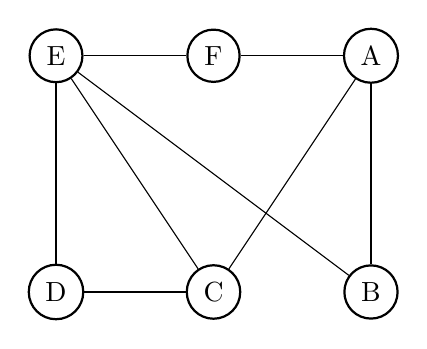
\begin{tikzpicture}
        \begin{scope}[every node/.style = {circle, thick, draw}]
            \node (A) at (2,0) {A};
            \node (B) at (2, -3) {B};
            \node (C) at (0, -3) {C};
            \node (D) at (-2, -3) {D};
            \node (E) at (-2, 0) {E};
            \node (F) at (0,0) {F};
        \end{scope}
        \begin{scope}
            \path[-] (E) edge (D);
            \path[-] (E) edge (C);
            \path[-] (E) edge (B);
            \path[-] (C) edge (D);
            \path[-] (B) edge (A);
            \path[-] (A) edge (C);
            \path[-] (A) edge (F);
            \path[-] (E) edge (F);
        \end{scope}
    \end{tikzpicture}
    \end{center}
	\begin{choices}
		\choice 32
		\choice 34
		\choice 36
		\choice 38
	\end{choices}

        \part[2] Which of the following statements are true for MST(Minimum Spanning Tree)?
        \begin{choices}
            \choice Suppose $G$ has multiple MSTs. For each minimum spanning tree $T$ of a graph $G$, there is a way to sort the edges of $G$ in Kruskal’s algorithm so that the algorithm returns $T$.
            \choice Prim's algorithm is a divide-and-conquer algorithm because it divides the graph into $S$ and $V-S$ then solve.
            \choice If we use binary heap to optimize Prim's algorithm when choosing the next edge, it will always have a better time complexity than the original algorithm on any graph.
            \choice If we add a new edge $e = (u,v)$ into a graph $G=(V,E)$ with unique MST to get a new graph $G' = (V,E\cup\{e\})$. There is at most $1$ edge difference between the MST of $G$ and $G'$.
        \end{choices}

\end{parts}


\newpage
\titledquestion{Huffman Coding}

After you compress a text file using the Huffman Coding Algorithm, you accidentally spill some ink on it and you find that one word becomes unrecognizable. Now, you need to recover that word given the following information:\\

    \textbf{Huffman-Encoded sequence of that word: } \\
    00001100111101\\
    \textbf{Frequency table that stores the frequency of some characters: }\\
    \begin{table}[!hbtp]
    \centering
    \begin{tabular}{|l|l|l|l|l|l|l|l|l|}
    \hline
    characters & b & e & i & k & m & t & x \\ \hline
    frequency  & 12 & 9 & 6 & 7 & 2 & 1 & 5 \\ \hline
    \end{tabular}
    \end{table}\\\\
\begin{parts}	
	\part[4] Please construct the binary Huffman Coding Tree according to the given frequency table and draw the final tree below.\\
	Note: The initial priority queue is given as below. When popping nodes out of the priority queue, the nodes with the same frequency follows ``First In First Out".
		
	\begin{table}[!hbtp]
	\centering
    \begin{tabular}{|l|l|l|l|l|l|l|}
    \hline
    \begin{tabular}[c]{@{}l@{}}t\\ 1\end{tabular} & \begin{tabular}[c]{@{}l@{}}m\\ 2\end{tabular} & \begin{tabular}[c]{@{}l@{}}x\\ 5\end{tabular} & \begin{tabular}[c]{@{}l@{}}i\\ 6\end{tabular} & \begin{tabular}[c]{@{}l@{}}k\\ 7\end{tabular} & \begin{tabular}[c]{@{}l@{}}e\\ 9\end{tabular} & \begin{tabular}[c]{@{}l@{}}b\\ 12\end{tabular} \\ \hline
    \end{tabular}
    \end{table}
    
    \begin{solution}
    \vspace{2in}
    \end{solution}

	\part[2] Now you can "decompress" the encoded sequence and recover the original word you lost. Please write the original word below.
	
	\begin{solution}
	    \vspace{0.5in}
	\end{solution}
	
\end{parts}

\newpage
\titledquestion{Binary Tree Practice}
\begin{parts}

\part[2] Consider the Binary Search Tree (BST) $T$ shown below, which satisfies the BST property (where each node's key is the integer value itself) but is not height-balanced. Identify all nodes that are not height-balanced.

\begin{center}
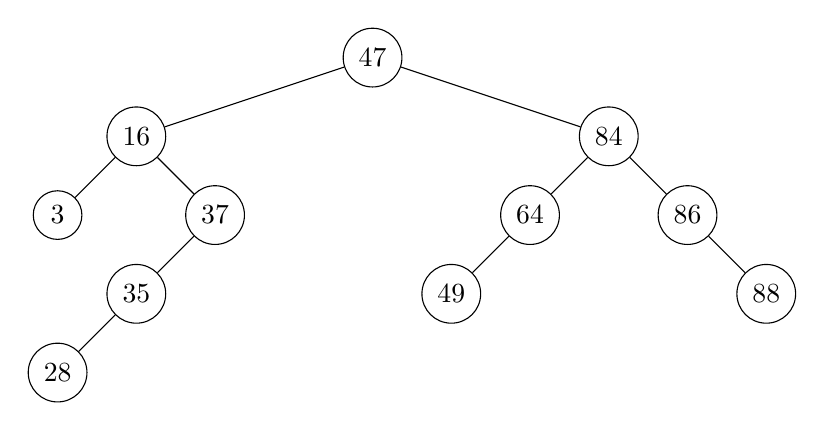
\begin{tikzpicture}[level distance=1cm,
            level 1/.style={sibling distance=2cm},
            level 2/.style={sibling distance=2cm},
            level 3/.style={sibling distance=2cm},
            every node/.style = {draw, circle}]
\node {47}
    child {node {16}
        child {node {3}}
        child {
            node {37}
            child {
                node {35}
                child { node {28} }
                child { edge from parent[draw=none] }
            }
            child { edge from parent[draw=none] }
        }
    }
    child { edge from parent[draw=none] }
    child { edge from parent[draw=none] }
    child {node {84}
        child {
            node {64}
            child { node {49} }
            child { edge from parent[draw=none] }
        }
        child {
            node {86}
            child { edge from parent[draw=none] }
            child { node {88} } 
        }
    };

\end{tikzpicture}
\end{center}

\begin{solution}
    \vspace{15pt}
\end{solution}

\part[5] Perform the following insertions and deletions, one after another in sequence on $T$, by adding or removing a leaf while maintaining the binary search tree property (a key may need to be swapped down into a leaf). For this part, do not use rotations to balance the tree. Draw the modified tree after each operation:
\begin{center}
    \texttt{T.insert(2)} \\
    \texttt{T.delete(49)} \\
    \texttt{T.delete(35)} \\
    \texttt{T.insert(85)} \\
    \texttt{T.delete(84)} \\
\end{center}

\begin{solution}
    \vspace{2.5in}

\end{solution}

\begin{solution}
    \vspace{8in}

\end{solution}

\end{parts}


\newpage
\titledquestion{Heap Practice}[8]
For each array provided:
\begin{enumerate}
\item Represent the array as a complete binary tree.
\item Determine if the tree is a max-heap, a min-heap, or neither.
\item If the tree is neither, convert it into a min-heap by repeatedly swapping adjacent items within the tree. Illustrate each swap by drawing the resulting sequence of trees, clearly indicating the swapped pairs on each tree.
\end{enumerate}

\begin{parts}
    \part 4, 12, 8, 21, 14, 9, 17

    \begin{solution}
        \vspace{2.5in}
    \end{solution}

    \part 700, 250, 23, 222, 10, 21
    \begin{solution}
        \vspace{2.5in}
    \end{solution}
    \newpage
    \part 2, 9, 13, 8, 0, 2
    \begin{solution}
       \vspace{3in}

    \end{solution}

\end{parts}


\newpage
\titledquestion{BST with Duplicates}

In our lecture, we require each BST node stands for a single unique element. However, in this question we are talking about BST with duplicated elements. That is, we need to maintain how many identical elements are in the BST. Now, each node may stands for multiple elements with the same value, and we call it the \ttt{count} of a node. Here we assume the value is \ttt{int} type. 

First we give the definition of our \ttt{Node} struct.

\begin{cpp}
struct Node {
    int val;    // The value of the node.
    int sumCount;    // The number of all elements in the sub-tree
    Node *left, *right; //the left and right child.
};
\end{cpp}

Note that \ttt{sumCount} stands for the number of all elements in the \textbf{entire sub-tree}, i.e. the sum of \ttt{count} in the entire sub-tree. You will see why we use this definition in the following questions.

For example, if root $r$ has two children $a$ and $b$, and neither $a$ nor $b$ has a child. Suppose $r\ttt{.count}=n_r$, $a\ttt{.count}=n_a$ and $b\ttt{.count}=n_b$. Then $r\ttt{.sumCount}=n_r+n_a+n_b$, $a\ttt{.sumCount}=n_a$, and $b\ttt{.sumCount}=n_b$.

\begin{parts}
    \part[3] After figuring out the definition of member variable \ttt{sumCount}, you need to design a function that calculates the \ttt{count} of a node, using \ttt{sumCount} variable. Please complete this function below, and make sure you do not access \ttt{nullptr}.

\begin{cpp}
// return how many elements a single node stands for
int get_count(Node *a){
    if(a == nullptr) return 0;
    int ans = /* (1) */ ;
    if(a->left != nullptr) ans = /* (2) */ ;
    if(a->right != nullptr) ans = /* (3) */ ;
    return ans;
}
\end{cpp}

\begin{solution}
    \vspace{1in}
\end{solution}


\part[4] Given a value $v$, we want to figure out how many elements are no more than $v$. Complete the function below, and make sure you do not access \ttt{nullptr}. You may use \ttt{get\_count} function if needed.
By calling \ttt{count\_no\_more\_than(root, v)}, we can get the number of such elements in the entire BST.

\begin{cpp}
// return how many elements are no more than v.
int count_no_more_than(Node *a, int v){
    if(a == nullptr) return 0;
    int ans = 0, tmp = 0;
    if (a->left != nullptr)
        tmp = /* (1) */ ;
    if(v < a->value)
        ans = /* (2) */ ;
    else if(v > a->value)
        ans = /* (3) */ ;
    else
        ans = /* (4) */ ;
    return ans;
}    
\end{cpp}

\begin{solution}
    \vspace{0.8in}
\end{solution}


\part[2] Now suppose you have finished the following two functions correctly. Given the root node of our BST, and two integers $l$ and $r$, how do you find out the number of elements in the range $[l,r]$? Use variables \ttt{root}, \ttt{l}, and \ttt{r}, and function \ttt{count\_no\_more\_than} to write an expression that computes the desired number.

\begin{cpp}
count_in_l_to_r = /* Your code */ ;
\end{cpp}

\begin{solution}
    \vspace{0.5in}
\end{solution}

\part[3] \textbf{True or False}

\begin{enumerate}
    \item[(i)] If we insert an element into our BST with duplicates, we may need to modify multiple nodes.
    \hfill \parbox[t]{1.50in}{
    \begin{oneparcheckboxes}
        \choice True
        \choice False
    \end{oneparcheckboxes}
    }
    
    \item[(ii)] If we delete a node in our BST with duplicates, the nodes that we need to modify are the nodes on the path from this node to the root.
    \hfill \parbox[t]{1.50in}{
    \begin{oneparcheckboxes}
        \choice True
        \choice False
    \end{oneparcheckboxes}
    }

    \item[(iii)] If we use member variable \ttt{count} instead of \ttt{sumCount}, we can still run \ttt{count\_no\_more\_than} in $O(h)$ time, where $h$ is the height of the tree.
    \hfill \parbox[t]{1.50in}{
    \begin{oneparcheckboxes}
        \choice True
        \choice False
    \end{oneparcheckboxes}
    }
\end{enumerate}



\end{parts}

\newpage
\titledquestion{MCTS practice}
In a Monte Carlo Tree, each node represents a state. In a node, using $a/b$ to represent its historical information, which means this state won $a$ times in $b$ times of search. In this problem, we use $UCB = \frac{a_i}{b_i} + \sqrt{\frac{\log_2(a_p)}{b_i}}$ , where node $p$ is the parent node of node $i$.
\newline
Here is a part of a Monte Carlo Tree, containing the first three layers (i.e. the fourth and deeper layers are omitted).

\begin{center}
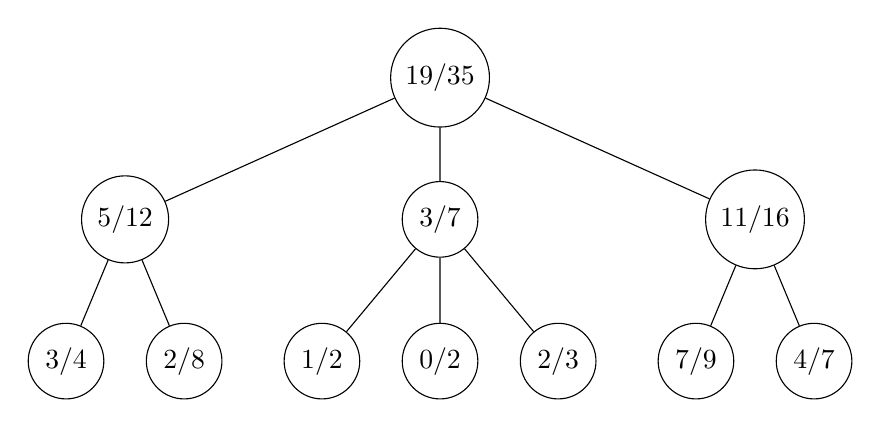
\begin{tikzpicture}[level distance=1.8cm,
            level 1/.style={sibling distance=4cm},
            level 2/.style={sibling distance=1.5cm},
            level 3/.style={sibling distance=1.5cm},
            every node/.style = {draw, circle}]
\node {$19/35$}
    child {node {$5/12$}
        child {node {3/4}}
        child {node {2/8}}
    }
    child {node {$3/7$}
        child {node {$1/2$}}
        child {node {$0/2$}}
        child {node {$2/3$}}
    }
    child {node {$11/16$}
        child {node {$7/9$}}
        child {node {$4/7$}}
    };

\end{tikzpicture}
\end{center}

\begin{parts}

\part[2] Given a Monte Carlo Tree above, which node in the third layer will be selected according to the MCTS algorithm?

\begin{choices}
    \choice $3/4$
    \choice $2/8$
    \choice $1/2$
    \choice $0/2$
    \choice $2/3$
    \choice $7/9$
    \choice $4/7$
\end{choices}

\part[4] After selecting a leaf node (deeper than the third layer), in the simulation step, the algorithm performs 5 simulations and wins 3 times. Please draw the new Monte Carlo Tree (the first three layers) after the Backpropagation step.

\begin{solution}
    \vspace{2in}
\end{solution}

\end{parts}


\end{questions}

\end{document}